\chapter{Arquitetura Emocional Constru\'ida} \label{ch:aec}

\section{Visão Geral}

A presente arquitetura construída foi pensada conforme mostrado na
Figura~\ref{fig:vasc}. Como se pode observar, o sistema é dividido em um
ambiente e em agentes. O ambiente utiliza as ontologias de preferências e de
rotinas para construir a visualização mostrada no capítulo~\ref{ch:cdu}. Dessa
forma, o que o usuário vê é exibido a partir da descrição da ontologia de
rotinas. Mais detalhes ver seção~\ref{ch:aec:ocu}. Já a de preferências,
explicada na seção~\ref{ch:aec:oda}, permite guardar junto dos objetos do
mundo virtual informações quando as mesmas forem estáticas e criar as
preferências dos agentes sobre essas informações.\dev{}
% O dev colocado acima se deve ao fato de a de preferencias ser guardarem
% informacoes, alem das proprias preferencias.

A segunda parte do sistema altera a mente dos atores agindo para acrescentar
anotações em suas percepções e para alterar local que essas crenças são
salvas. A mente dos atores é chamada agente e eles recebem via percepção as suas
preferências e rotinas\dev{}. Essa escolha foi feita para permitir que a
escolha do que fazer seja toda ela escrita em código\dev{} da plataforma
\emph{Jason}. As emoções são concluídas pelo agente através de ontologia
(ver seção~\ref{ch:aec:omce}) e, portanto, a base de crenças padrão da
plataforma foi estendida para consultar, guardar e recuperar os dados
diretamente nessa quando a crença for relevante. Sendo assim, é como se
houvesse dois níveis. O primeiro formado pela ontologia e o segundo pela base
de crença padrão.

\begin{figure}
  \centering
  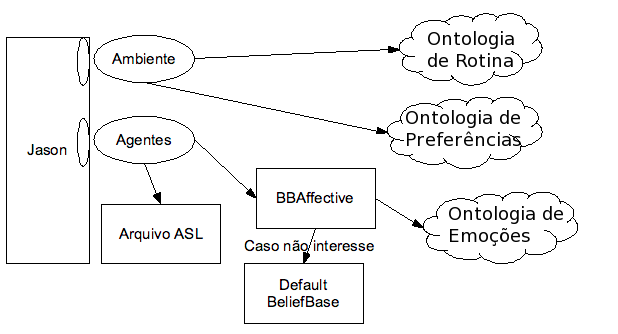
\includegraphics[width=10cm]{figuras/visao-geral.png}
  \caption{Visão abstrata do sistema construído.}
  \label{fig:vasc}
\end{figure}

\section{Ontologia do Modelo Cognitivo Emocional} \label{ch:aec:omce}

A fundamentação do modelo afetivo sendo utilizado aqui é o proposto por
\citet{ortony1988cse} e encontra-se explicado na seção \ref{ch-ca-mce}. A
ontologia proposta tinha como ideia inicial não utilizar regras, porém como
pode ser observado na Tabela~\ref{tab:oa:geral} foi necessário a criação de
regras para suportar o raciocínio no nível de indivíduo corretamente. As
regras que ajudam a conclusão das relações \emph{hasKnow}, \emph{hasFriend} e
\emph{hasEnemy} são diferentes das demais por causa que elas tem como
característica operar no domínio e na imagem da classe \emph{Agent}. Por
exemplo, se John avalia que se relaciona bem com Jose então John
\emph{hasFriend} Jose. Note que o contrario não é necessariamente verdade, o
Jose pode apenas saber que conhece o John então Jose \emph{hasKnow} John.

\begin{table}[h]
	\caption{Ontologia proposta com expressividade: ALCHIN(D).}
	\label{tab:oa:geral}
	\begin{center}
	\begin{tabular}{|c|c|}
	%\begin{tabular}{|p{34mm}|p{50mm}|p{50mm}|}
		\hline
		Descrição & Quantidade \\ \hline
		Classes &  45 		\\ \hline
		Propriedade de Objetos & 16 \\ \hline
		Propriedade de Dados & 14 \\ \hline
		Indivíduos &  0		\\ \hline
		Regras & 7 \\ \hline
	\end{tabular}
	\end{center}
\end{table}

Na Figura~\ref{fig:rlocc} são mostradas as regras desenvolvidas, elas dependem
que os indivíduos da ontologia sejam marcados como diferentes um dos outros.
Assim, recomenda-se fortemente que quando registrar um indivíduo da classe
\emph{Object} ou \emph{Agent} que a informação de igualdade ou diferenciação
seja preenchida\dev{}. Assim, se evita que o raciocinador conclua que não
conhece a resposta e chegue a uma conclusão não esperada.

\begin{figure}[b]
  \centering
  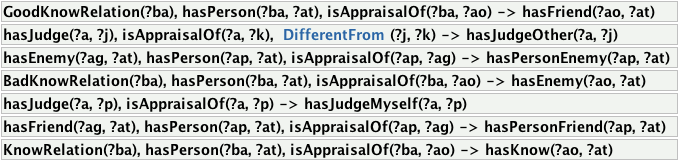
\includegraphics[width=14cm]{figuras/rules-LOCC.png}
  \caption{Regras da ontologia proposta.}
  \label{fig:rlocc}
\end{figure}

A Figura~\ref{fig:kplocc} mostra a árvore de relações que tem como imagem
dados ou instâncias (objetos). Ao se comparar as Figuras~\ref{fig:rlocc}
e \ref{fig:kplocc} se chega a conclusão que as propriedades que as
regras concluem não precisam ser configuradas pelo usuário. Assim, ao invés de
16 propriedades de objetos conforme informado na Tabela~\ref{tab:oa:geral}
apenas 9 precisam ser conhecidas. Dessas, a propriedade menos utilizada é a
\emph{hasSomething} que serve para indicar genericamente o que esta sendo avaliado. Note que
\emph{hasPerson} deve ser usado quando o indivíduo em avaliação for um membro
da classe \emph{Agent}. Já, a relação \emph{hasJudge} serve para indicar que o
membro da classe \emph{Object} esta sendo avaliado pela sua responsabilidade.
Por exemplo, Millie tem uma avaliação julgando seu carro com uma valoração
positiva.

\begin{figure}[b]
  \centering
  \begin{tabular}{cc}
  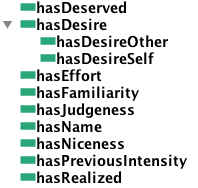
\includegraphics[height=4cm]{figuras/dataProperty-LOCC.png} & 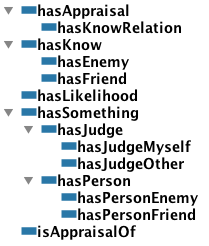
\includegraphics[height=5cm]{figuras/objectProperty-LOCC.png} \\
  (i) Relações de dados & (ii) Relações de Objetos
  \end{tabular}
  \caption{As relações existentes na ontologia proposta.}
  \label{fig:kplocc}
\end{figure}

Todos os dados numéricos da ontologia são inteiros. Isso foi feito com a
finalidade de permitir que o usuário normalize\dev{} o número obtido da
maneira que desejar. Além disso, foi tomada a decisão de não especificar o
domínio da maioria das propriedades por causa que isso forçaria um
enquadramento em classes não desejadas. Por exemplo, se a relação
\emph{hasLikelihood} tiver o domínio \emph{ConsequenceForSelf} e existir um
indivíduo com somente essa relação então o mesmo seria enquadrado no conceito
\emph{ConsequenceForSelf}. Mas, o correto nesse caso seria não ser concluído nada,
ou seja, pertencer à classe \emph{Thing}.

A estrutura da ontologia pode ser visualizada na
Figura~\ref{fig:tlocc}~(pág.~\pageref{fig:tlocc}). Além disso, pode ser
recomendável olhar a
Figura~\ref{fig:occ_model}~(pág.~\pageref{fig:occ_model}) do modelo \occ
durante o resto da discussão dessa seção. Os sub-conceitos de \emph{Emotion}
correspondem aos três ramos do modelo original.
O ramo \emph{ActionsOfAgents} julga a responsabilidade e o quanto o agente que
realizou uma ação ou evento se desviou do esperado, o de
\emph{ConsequencesOfEvents} julga a consequência de um evento e
\emph{AspectsOfObjects} julga a atração para com um objeto.

O primeiro ramo a ser abordado é, o menos cognitivo, \emph{AspectsOfObjects}.
As emoções desse tipo são relacionadas com atratividade e familiaridade.
Entretanto, essas duas relações foram consideradas equivalentes porque o
importante, para o modelo, é quando ambas são positivas ou ambas negativas.
Assim sendo, uma pode assumir os dois papeis sem maiores penalidades e
simplificando a modelagem. A emoção \emph{Hate} é modelada como tendo a
propriedade de familiaridade (\emph{hasFamiliarity}) com valores negativos,
enquanto a emoção \emph{Love} tem valoração dessa mesma propriedade positiva.
Caso o valor seja zero, nada pode ser concluído.

Cabe notar que parece estranho uma emoção \emph{Love} com um objeto, porém
essa emoção foi escolhida por quem montou o modelo para representar seu tipo
por ser a mais forte de sua categoria. Assim, níveis menores implicam em
outros tipos de emoção. Além disso, agentes
podem ser vistos como objetos quando se esta avaliando a sua atração. Assim,
todo agente (\emph{Agent}) é um objeto (\emph{Object}). Por exemplo, John esta
apaixonado pela Millie (\emph{Agent} visto como \emph{Object}) ou John tem
repulsa por televisão.

O segundo conceito, chamado \emph{ActionsOfAgents}, pode ser pensado como
um ramo que julga a responsabilidade por uma determinada ação ou evento.
Assim, esse ramo é capaz de gerar emoções de: Admiração (\emph{Admiration}),
Orgulho (\emph{Pride}), Vergonha (\emph{Shame}) e Reprovação
(\emph{Reproach}). Por exemplo, Jose possui orgulho por cozinhar ou Dilu
reprova Jose porque ele come carne.

Na definição, as emoções de orgulho e vergonha podem acontecer mesmo quando se
esta avaliando ações de outras pessoas. Por exemplo, Dolores tem vergonha de
sua mãe que não cozinha. Essa conclusão é possível por causa de uma relação
que eles propõem de empatia. Entretanto, como em nenhum outro momento, eles
dão mais detalhes sobre essa empatia foi resolvido considerar que vergonha e
orgulho são emoções sentidas somente quando o agente esta avaliando a si mesmo
e, dessa forma, o exemplo anterior não é possível no sistema desenvolvido. \dev{}
% dev -> poderia ter sido usado float e ter feito 1 (para si) e 0 (para outro)

As emoções que julgam responsabilidade são definidas como tendo uma relação de
julgamento (\emph{hasJudge}) e uma relação que mapeia o valor do julgamento
(\emph{hasJudgeness}) que representa o quanto o agente se desviou do
comportamento esperado, isto é, em casos de aprovação é um valor positivo e em
casos de reprovação é um valor negativo. Todavia, isso ainda não permite
diferenciar a emoção de admiração da emoção de orgulho ou a reprovação da de
vergonha. Essa distinção é possível ao se dividir a relação de julgamento com
duas sub-relações: tem auto-julgamento (\emph{hasJudgeMyself}) e tem
julgamento de outro (\emph{hasJudgeOther}).

A utilização de sub-propriedade torna possível escrever a ontologia da maneira
esperada suprimindo o problema. Entretanto, para o usuário pode se tornar
complicado ter que lembrar quando utilizar uma sub-propriedade ou outra.
Assim, foi resolvido deixar o usuário sempre utilizar a relação de julgamento
(\emph{hasJudge}) e via 2 regras inferir se é um auto-julgamento ou o
julgamento de outra pessoa. Para essas regras funcionarem da maneira correta,
o usuário deve declarar que os agentes ou objetos são diferentes uns dos
outros. Caso isso
não ocorra, o sistema considera que não há informação para verificar se um
indivíduo é igual ou diferente e conclui que não conhece a resposta. Além
disso, a relação de julgamento tem como imagem o conceito \emph{Object}. Dessa
forma, os exemplos anteriores são todos válidos.

Cabe salientar que toda avaliação tem pelo menos duas relações. A primeira
relação serve para conhecer quem esta avaliando (\emph{isAppraisalOf}) e a
outra serve para indicar quem ou o que esta sendo avaliado
(\emph{hasSomething}). Essa pode não ser informada explicitamente porque pode
ser concluída quando usada uma de suas sub-relações. O último ramo, chamado de
\emph{ConsequencesOfEvents} é dividido em: \emph{ConsequencesForSelf} e
\emph{ConsequencesForOthers}. Toda essa divisão foca na consequência de um
evento ou ação realizado por algum agente. Por exemplo, Dilu tem pena
de Jose, Jose tem esperança de ser promovido, John tem satisfação por
estar almoçando ou Millie esta alegre por cozinhar.

\begin{wrapfigure}{r}{0.4\textwidth}
  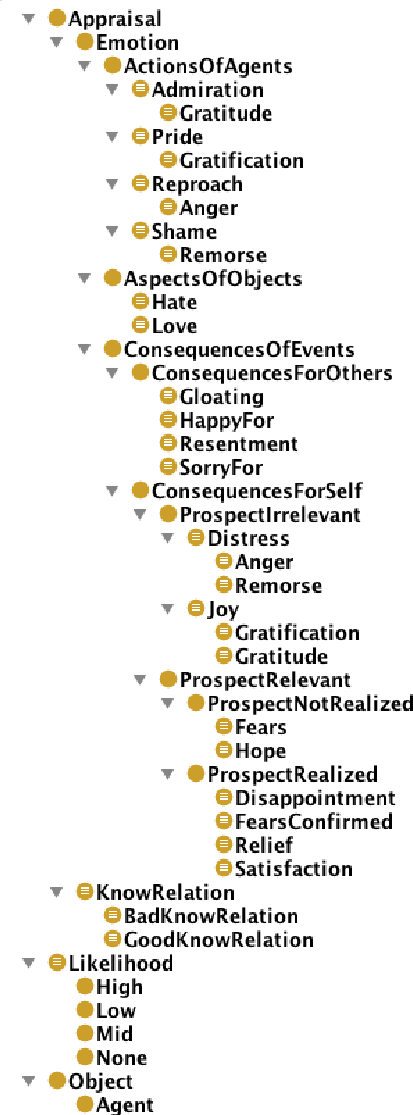
\includegraphics[height=149mm]{figuras/hierarquiaLOCC.png}
  \caption{Taxonomia da ontologia proposta baseado no modelo.}
  \label{fig:tlocc}
\end{wrapfigure}

A \emph{ConsequencesForOthers} expressa 4 emoções: \emph{HappyFor},
\emph{SorryFor}, \emph{Gloating} e \emph{Resentment}. Na definição, essas
emoções dependem: do grau de desejabilidade do avaliador para com o outro; do
grau de desejabilidade que se presume que o outro tenha; do grau de
merecimento do evento; e, do tipo de relacionamento com a pessoa. Na ontologia
proposta, a principal diferença com o modelo \occ é que foi considerado
que o grau de desejabilidade do avaliador para com o outro e o grau de
merecimento do evento são os mesmos. Dessa forma, se pode utilizar apenas três
relações para descrever as 4 emoções.

A relação de merecimento (\emph{hasDeserved}) e relação de desejabilidade
presumida (\emph{hasDesireOther}) são avaliadas de acordo com sua valoração
positiva ou negativa. A relação \emph{hasPerson} liga o outro indivíduo
sendo avaliado com a avaliação. Para se ter o conhecimento esta sendo julgado
é amigo (\emph{GoodKnowRelation}) ou inimigo (\emph{BadKnowRelation}), esses
conceitos foram criados e precisam ser configurados para cada um dos agentes
em questão. O mesmo pode declarar que só conhece uma pessoa, que conhece e é
um amigo ou que conhece e não gosta dela (inimiga). Entretanto, quem precisa
dessa informação é o conceito de avaliação quando as relações
\emph{hasPersonEnemy} e \emph{hasPersonFriend} precisam ser descobertas.

\emph{ConsequencesForSelf} se divide entre consequências de eventos com
probabilidade relevante (\emph{ProspectRelevant}) e irrelevante
(\emph{ProspectIrrelevant}). Cabe salientar que esses dois conceitos se
relacionam com probabilidade (\emph{hasLikelihood}), entretanto enquanto o
primeiro conceito se relaciona com a parte não nula. A outra se relaciona
somente com essa. Dessa forma, ambos os conceitos são disjuntos. A classe de
probabilidade relevante pode ser dividida ainda entre possibilidade não
realizada (\emph{ProspectNotRealized}) e realizada (\emph{ProspectRealized}).

As emoções \emph{Hope} e \emph{Fear} fazem parte do conceito
\emph{ProspectNotRealized}. Esse conceito usa as relações \emph{hasLikelihood}
e \emph{hasDesireSelf}. Essa última propriedade é um número que
representa o desejo de se obter ou repudiar o evento. Além disso, quando o
evento ocorre a emoção atual pode virar uma emoção do conceito
\emph{ProspectRealized}, isto é, \emph{Fear} pode virar ou
\emph{FearsConfirmed} ou \emph{Relief} e \emph{Hope} pode virar ou
\emph{Satisfaction} ou \emph{Disappointment}.

O conceito \emph{ProspectRealized} não se relaciona em nenhum momento com a
relação \emph{hasLikelihood} porque o evento já aconteceu ou não vai mais
acontecer. Assim, ele possui três relações distintas das anteriores, a
primeira é o grau de realização de um evento (\emph{hasRealized}), isto é, a
visão do agente sobre como a consequência do evento aconteceu. A segunda
relação \emph{hasPreviousIntensity} recebe a valoração da emoção de medo ou
esperança do evento que tinha probabilidade e serve para saber se o evento era
um evento bom (esperança) ou ruim (medo). Já, a terceira \emph{hasEffort}
tenta estimar o grau de esforço que foi dispendido para a atração ou repulsa
da consequência do evento.

O conceito \emph{ProspectIrrelevant} é parecido com o conceito
\emph{ProspectRelevant} com a diferença que a relação \emph{hasLikelihood} vai
somente para valores nulos. Alem disso, as emoções desse conceito e do
\emph{ActionsOfAgents} podem ser misturadas formando conceitos compostos.
A composição é quando uma emoção pode ser encaixada em mais de uma emoção
como no caso de se estar alegre (\emph{Joy}), orgulhoso (\emph{Pride}) e
gratificado (\emph{Gratification}). Por fim, o conceito \emph{Setup}
é o utilizado para manter junto da ontologia criada o limite mínimo para uma
emoção virar sentimento\dev{}.

%a transferencia eh feita pelo sistema;
%os dados sao carregados para memoria e eliminados;
%conforme reparado nao ha decaimento da emocao, a mesma eh instantanea;
%2345678901234567890123456789012345678901234567890123456789012345678901234567890

\section{Ontologia de Comportamento Urbano} \label{ch:aec:ocu}

O presente trabalho foca no comportamento de personagens. Dessa forma, uma
ontologia de comportamento urbano tenta descrever a vida normal que um
personagem leva. De outro modo, isso pode ser visto como a rotina regular que
o ator possui em sua cidade virtual.

\begin{figure}
  \centering
    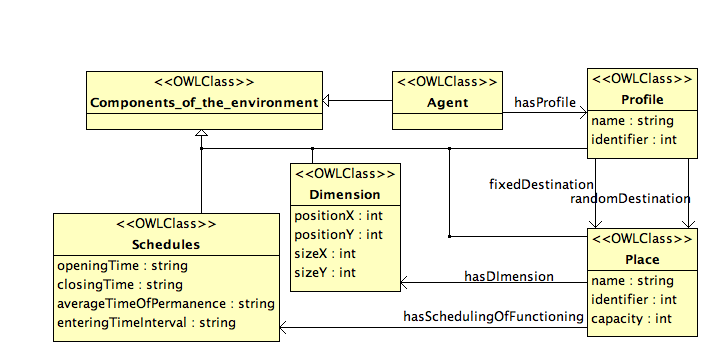
\includegraphics[width=150mm]{figuras/uem-tbox.png}
  \caption[T-Box baseado no modelo de ambiente urbano.]{T-Box baseado no modelo de ambiente urbano \cite{paiva2005ontology}.}
  \label{fig:UEM:TBOX}
\end{figure}

A Figura~\ref{fig:UEM:TBOX} demostra a ontologia, criada por
\citet{paiva2005ontology}, que será utilizada. As relações de generalização
possuem a mesma semântica que na UML, as relações direcionais são relações
binárias entre as instâncias das classes. Na figura, \emph{Agent} se relaciona
com o conceito \emph{Profile} para determinar o tipo de agente. O
\emph{Profile} do agente pode variar entre alguns tipos especificados pelo
usuário que podem possuir destinos fixos (usuais) ou destinos randômicos
(eventuais).

Esses locais são definidos pelo conceito \emph{Place} que contêm
uma descrição de sua capacidade (quantidade máxima de atores), dimensão
(acessível por relação) e horário de funcionamento (acessível por relação). O
conceito de \emph{Dimension} guarda a posição e o tamanho nos eixos X e Y. Já,
o conceito de \emph{Schedules} possui o horário de abertura e fechamento,
intervalo de entrada e tempo médio de permanência.

Além disso, o conceito \emph{Components\_of\_the\_environments} esta sendo
pensando como um sub-conceito do conceito \emph{Setup} na ontologia
desenvolvida por causa que esse representa as configurações gerais.
%
%Essas configurações gerais são carregadas, normalmente, em outras partes do
%sistemas e então eliminadas por causa que elas não influenciam as emoções
%diretamente.
Fora isso, foi introduzido uma nova relação chamada \emph{hasCharacter} que
mapeia o conceito de agente do modelo \occ para o conceito apresentado aqui.
Dessa forma, um agente na ontologia do
modelo \occ pode descobrir seu perfil e descobrir seus locais visitados
regularmente. O conceito de \emph{Place} pode ser pensado, como veremos
adiante, como um ``objeto inteligente''.

Essa ontologia é utilizada no presente trabalho de duas formas. A primeira
forma de utilização é para desenhar um mapa 2D do ambiente que os agentes
atuam. Isso é permitido porque o conceito \emph{Place} relaciona-se com o
\emph{Dimension}. Assim, todos os itens do mapa são retângulos. A outra forma
de utilização é a que trouxe a ontologia para o trabalho e é definir que um
agente tenha sua rotina descrita e disponibilizada pelo ambiente. Para o
ambiente disponibiliza-la via percepção, no ambiente simulado construído cada
dia simulado equivale a aproximadamente 96 ciclos. Isso quer dizer que cada
passo simulado seria em torno de 15 minutos de um dia. Dessa forma, o ambiente
é responsável por conhecer que dia é e informa-lo junto das rotinas daquele
dia para cada agente.

\section{Ontologia de Preferências} \label{ch:aec:oda}

\citet{doyle1998annotated} propuseram que o mundo contivesse uma série de
anotações nos objetos. Assim, o agente poderia conhecer apenas a forma de
questionar os objetos sobre suas formas de usar, suas descrições e suas outras
características. Esse conceito veio do conceito \emph{affordance} que se
refere a propriedade de um objeto que dita como o mesmo será utilizado.
Dessa forma, uma cadeira tem a propriedade de ser sentada e uma porta tem as
propriedades de ser aberta ou ser fechada.

Assim, eles utilizaram 5 tipos de anotações: (i) anotações emocionais,
explicam como um agente responde ``emocionalmente''; (ii) anotações de
resposta, explicam como o agente deve reagir ao evento no ambiente que pode ser
uma ação especifica ou uma sugestão de crença; (iii) anotações de resolução de
problemas, descreve o estado do problema e permite anotar dicas que o ator
talvez fale ou realize; (iv) anotações de papel, informam o agente sobre ações
relevantes para determinados trabalhos no mundo; (v) anotações de jogo,
descrevem o estado do jogo permitindo sugerir movimentos.

\citet{kallmann1999modeling} explicaram uma ideia similar, os objetos no mundo
são os responsáveis por proverem para o personagem o como ele deve ser usado.
Por exemplo, durante a animação do personagem estar abrindo uma porta, quem esta
no controle do ator é o ``agente'' que controla a porta. O agente do
personagem delega a responsabilidade da animação para o agente do objeto por
causa que o mesmo é o único que sabe como realizar a animação de abertura ou
fechamento da porta. Esses objetos, denominados objetos inteligentes, precisam
ter um determinado nível de conhecimento sobre o personagem.

De uma maneira similar, o conceito de artefatos que possuem propriedades
observáveis e utilizáveis foi criado por \citet{ricci31cartago}. Por exemplo,
uma porta pode ter como propriedade observável seu estado (estar aberta ou
estar fechada) e ação possível ou propriedade utilizável ser aberta ou ser
fechada. Essas ações podem ficar disponíveis conforme o estado atual do
objeto, mas o controle da disponibilidade e da ação é do próprio objeto por
que é ele que sabe como realizar a ação propriamente dita. O agente unicamente
diz de alguma forma que o objeto tem que realizar tal ação. Nesse trabalho,
não é mencionado que o agente pode ser temporariamente controlado por
objetos.

\begin{figure}
  \centering
    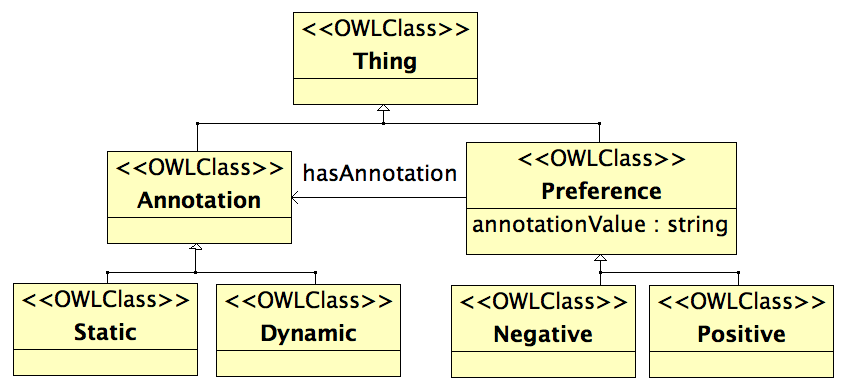
\includegraphics[width=130mm]{figuras/preferences.png}
  \caption{T-Box da ontologia de preferências proposta.}
  \label{fig:preferences}
\end{figure}

A ontologia proposta para as preferências pode ser vista na
Figura~\ref{fig:preferences}. Como pode ser observado, foi criado dois
conceitos principais \emph{Annotation} e \emph{Preference}. O conceito
\emph{Annotation} é utilizado para representar características de determinadas
coisas. Essas características podem ainda ser categorizadas entre as que mudam
e não mudam durante a simulação. O sub-conceito \emph{Dynamic} representa as
características dinâmicas, isto é, as características que podem ser alterados
durante a ``vida'' do objeto. O sub-conceito \emph{Static} representa as
características que não podem ser alteradas depois da criação do objeto. O
calor e o dono são exemplos de características dinâmicas, enquanto o nome e a
capacidade total são exemplos de características estáticas.

O conceito \emph{Preference} é usado para representar as preferências por
determinadas características ou anotações. A preferência define como uma entidade ou
agente é atraído por determinada característica, por exemplo algumas pessoas
gostam de calor e outras não. Assim, as pessoas que gostam de calor são
atraídas pela valoração positiva da anotação de calor. Já, as pessoas que não
gostam de calor são atraídas pela valoração negativa. Dessa forma, os
sub-conceitos da preferência representam sempre valores que fazem o agente ser
atraído pelo objeto e repelido caso contrário.

Entretanto, esse exemplo não funciona para todos os casos. Por exemplo, um
agente tem conhecimento de seu nível de energia e este é sempre positivo. Para
resolver esse problema foi criada a relação \emph{hasAnnotationValue}
representada na Figura~\ref{fig:preferences} pelo atributo
\emph{annotationValue}. Sendo assim, é possível descrever que um agente com
nível de energia abaixo de um determinado limite é atraído pelo seu centro de
controle.

Essas anotações em objetos foram planejadas para serem colocadas pelo ambiente
nos objetos e nos agentes. As anotações em agentes permitem que outros saibam
o que o agente esta fazendo e como ele parece de forma similar aos objetos. As
preferências também são disponibilizadas em formas de percepção, mas o usuário
que deve criar regras ou planos no \jason para montar as relações usadas pela
afetividade.

\section{Integrando a Plataforma \jason com as ontologias} \label{ch:p:ipjo}

As ontologias explicadas, nas seções anteriores, foram planejadas para serem
usadas como módulos. Sendo assim, as ontologias explicadas anteriormente
podem ser usada sem implicar no uso das demais. Cabe salientar que elas podem ser
usadas tanto pelo agente quanto pelo ambiente.

No capítulo~\ref{ch:cdu}, um dos agentes utiliza a ontologia afetiva e o
ambiente utiliza a ontologia de preferência e rotinas. Assim, um lugar
definido pelo conceito \emph{Place} pode possuir a relação \emph{hasSetup} visando
duas coisas. A primeira é determinar as anotações existentes em um objeto que
esta em um determinado lugar. A segunda é indicar que objetos fazem parte dos
lugares para que o agente tenha uma especie de mapa abstrato do local, por
exemplo o agente sabe que a sala 1 possui um armário, dois criados mundos, 2
duas camas e duas portas. Mas, não conhece nenhuma das anotações desses
objetos no mapa abstrato sendo necessário ir até eles para tal.

\begin{figure}[b]
  \centering
  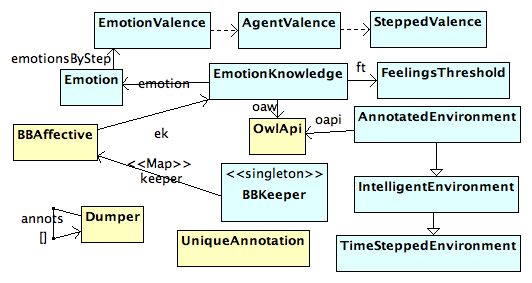
\includegraphics[width=8cm]{figuras/implementacao-15dez2011.png}
  \caption{Diagrama de classes do sistema.}
  \label{fig:dcs}
\end{figure}

Na figura~\ref{fig:dcs} pode ser observado as classes desenvolvidas para
realizar a integração das ontologias com os agentes \emph{Jason}. Para essas classes
serem usadas, o agente deve ser configurado para utilizar a classe
\emph{BBAffective} como base de crença e a \emph{UniqueAnnotation} como classe
do agente para a implementação da afetividade funcionar perfeitamente. Essas
configurações podem ser feitas conforme explicado na
seção~\ref{sec-jason-architecture} (pág.~\pageref{sec-jason-architecture}) e
demostrado na seção~\ref{ch:cdu:tbc} (pág.~\pageref{ch:cdu:tbc}).

A classe \emph{UniqueAnnotation} é responsável por garantir a não duplicidade
de anotações. Assim, quando se insere por algum motivo duas vezes a mesma
anotação apenas valerá a última. Já, a responsabilidade da classe
\emph{BBAffective} é manter as crenças dos agentes e atender as solicitações
da plataforma \jason sobre a manipulação dessas em dois níveis. O primeiro
nível é a ontologia e o segundo é a base de crença padrão que é utilizada
quando o elemento não é considerado relevante para o primeiro nível. A
relevância é descoberta consultando os conceitos e propriedades existentes na
ontologia, por exemplo instâncias de conceitos são crenças no formato
``nomeDoConceito(nomeDaInstancia)'' e relações são similares
``nomeDaRelacao(nomeDaInstanciaDominio, Imagem)''. A base de crenças delega
todo o assunto relacionado com as crenças da ontologia para a classe
\emph{EmotionKnowledge}. Essa é responsável por conhecer todo o assunto
relacionado com as emoções e sentimentos e delega a manipulação e consulta da
ontologia, propriamente dita, para a classe \emph{OwlApi}.

A classe \emph{SteppedValence}, \emph{AgentValence} e \emph{EmotionValence}
são extensões da classe \emph{HashMap}. A primeira usa como chave o passo da
simulação e obtém um número que representa a valência da emoção no momento. A
próxima, usa o nome do agente como chave para obter uma instância da
\emph{SteppedValence}. A terceira, devolve uma instância da segunda
baseando-se no nome da emoção. Esse último \emph{hash} é mantido na classe
\emph{Emotion} juntamente com uma lista de todas as emoções possíveis
retiradas da própria ontologia.

Conhecer o limite mínimo para uma emoção ser sentida e virar sentimento é de
responsabilidade da classe \emph{FeelingsThreshold}. As classes de ambiente,
isto é, as classes que possuem \emph{Environment} no nome são responsáveis por
manter os passos de simulação com um tempo máximo, conhecer a quantidade de
agentes que tem que esperar responderem para dai ir ao passo de simulação
seguinte e carregar as ações definidas do ambiente a partir do pacote
especificado estendendo a classe \emph{ActionLoader} (não desenhada). O
conhecimento do formato das crenças e como converte-lo para o formato interno
com a finalidade de proteção de mudanças da plataforma \jason é
responsabilidade da classe \emph{Dumper}. Já, a classe \emph{BBKeeper} é um
\emph{singleton} e é responsável por conhecer todas as instâncias da classe
\emph{BBAffective}. Essa classe precisa ser um \emph{singleton} para, dessa
forma, poder em qualquer ponto do código as emoções ou outras crenças serem
consultadas.

Na figura~\ref{fig:addBelief} esta representado o processo de inserção de
uma crença. No UML a possibilidade de se colocar guardas que são etiquetas que
dizem a condição para o código ser executado. Essas guardas foram colocadas
perto de um quadrado para simbolizar que todas as chamadas feitas dentro dele
estão relacionadas aquelas condições. Dessa forma, quando estiver sendo
inserida uma crença de percepção com o termo diferente de ``step'' nenhum código será
executado pelo diagrama e o insere no segundo nível.

A chamada do \jason para a função \emph{add} não se encontra representada na
figura~\ref{fig:addBelief}, porém essa função chama uma outra de mesmo nome e
quando essa retorna falso é chamada a função \emph{add} da instância
\emph{next}. Cabe chamar atenção que quando uma percepção esta sendo inserida,
ela é sempre posta no segundo nível da base de crença. Entretanto, quando o
termo da crença é ``step'' aproveitamos para realizar o processo de
sumarização que calcula e guarda a potência da emoção na classe
\emph{Emotion}. Além disso, se aproveita o momento para obter e inserir na
base de crenças padrão os sentimentos que acabaram de sofrer atualização em
seus valores.

Agora quando o esta sendo feita uma inserção de uma crença que não é uma
percepção, é feita a verificação se ele é relevante. Caso ele seja considerado
irrelevante, a crença sera inserida no segundo nível. Entretanto, se ele for
considerado relevante então será feita a recuperação do elemento atualmente
armazenado e, após isso, é feita a inserção das novas anotações nesse
elemento. Se o elemento não existir na base de crenças então esse último
procedimento é ignorado, porém ele é necessário para haver a correta
atualização das anotações. Por fim, a crença é transformada no tipo interno e
enviado para ser acrescentado na ontologia.
O processo de inserção na ontologia depende se o que esta sendo inserido é uma
instância de objeto ou de propriedade de objeto ou de propriedade de dados.

A potência de uma emoção é calculada usando as relações de dados de indivíduos
classificados como sendo uma avaliação. Dessa forma, a potência é a soma de
todas as relações de um mesmo indivíduos. Se houver interesse em conhecer em
por menores o código, ele encontra-se disponível no
\emph{GitHub}\footnote{http://github.com/rlucca/Maro}.

\begin{figure}
  \centering
  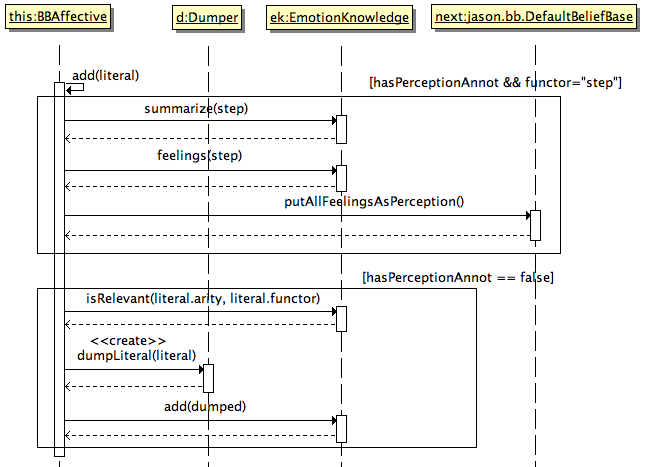
\includegraphics[width=12cm]{figuras/addB.png}
  \caption{Diagrama de sequência para adicionar uma crença.}
  \label{fig:addBelief}
\end{figure}

